\section{Architecture of the game}
In this section we will look at the overall architecure of the different components involved in the game.
\begin{figure}[H]
    \centering
    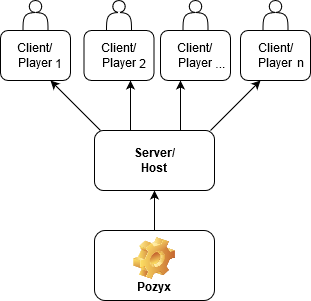
\includegraphics[width=0.6\linewidth]{Architecture.png}
    \caption{The different components of the game}
    \label{fig:architecture}
\end{figure}
In \autoref{fig:architecture} an illustration of how we imagine the different components of the game are going to work together is shown.
The Pozyx component is responsible for providing the positional data to the host. 
Each client/player is equipped with one of the tags which tracks their position on the field. 
The playing fields dimensions will be the distance between the anchors. 
The host has the positional data for each client, but it will also need to know which of the tags each client is equipped with.
The host will then continuosly transfer positional data to the clients which will also include the tag id that belongs to that client.
Each client will be running an instance of the game, and with use of the positional data it can render the playing field, the ball and each of the players.
